\section{RQ4: Final Comparison}
\label{sec:rq4}

The final comparison runs three algorithms for 60 seconds with seeds that were not used before: the original implementation of POEMS with the parameters of the original edition ({\em original POEMS}), POEMS with the corrections, the array evaluation and the modifications chosen in Section~\ref{sec:rq2} ({\em improved POEMS}), and LA-POEMS in the configuration chosen in Section~\ref{sec:rq3}. The held-out instances were not used before this comparison.

\subsection{Tuning Benchmarks}

Table~\ref{tab:final} shows the results on the eight benchmarks used for tuning. All three algorithms find the same floorplan of apte (0.78\,\%) in every run. On the other seven benchmarks, LA-POEMS is significantly better than the original POEMS, with $\hat{A}_{12} \geq 0.98$: almost every run of LA-POEMS ends with less dead space than every run of the original algorithm. It reduces the mean dead space by 28\,\% on xerox, by 57--65\,\% on hp, ami33, ami49 and n100 and by 69--73\,\% on n200 and n300, from 10--11\,\% to 2.8--3.4\,\%. It finds the best known floorplan of hp (1.32\,\%) in seven of eight runs and that of xerox (2.30\,\%) in four. The improved POEMS, which differs from the original algorithm by the corrections, the faster evaluation and $G = 100$, is itself significantly better than the original POEMS on all seven benchmarks: it reduces the dead space by 44--58\,\% on six of them and by 12\,\% on xerox. LA-POEMS is significantly better than the improved POEMS on five benchmarks, by 11--38\,\% ($\hat{A}_{12} = 0.83$--$1$), and better but not significantly on hp and ami49 ($\hat{A}_{12} = 0.58$ and 0.80).

\begin{table}
\centering
\footnotesize
\setlength{\tabcolsep}{4pt}
\begin{tabular}{@{}lcccrr@{}}
\toprule
 &  &  &  & \multicolumn{2}{c}{$\hat{A}_{12}$ of LA-POEMS vs.} \\
Benchmark & original & improved & LA-POEMS & original & improved \\
\midrule
apte & $0.78_{\pm 0.00}\ (0.78)$ & $0.78_{\pm 0.00}\ (0.78)$ & $0.78_{\pm 0.00}\ (0.78)$ & 0.50 & 0.50 \\
xerox & $3.23_{\pm 0.16}\ (3.16)$ & $\mathbf{2.85_{\pm 0.39}\ (2.34)}$ & $\mathbf{2.32_{\pm 0.02}\ (2.30)}$ & 1.00 & 0.91 \\
hp & $4.57_{\pm 1.23}\ (2.28)$ & $\mathbf{2.13_{\pm 1.46}\ (1.32)}$ & $1.62_{\pm 0.79}\ (1.32)$ & 0.98 & 0.58 \\
ami33 & $3.31_{\pm 0.56}\ (2.33)$ & $\mathbf{1.86_{\pm 0.36}\ (1.37)}$ & $\mathbf{1.16_{\pm 0.40}\ (0.63)}$ & 1.00 & 0.91 \\
ami49 & $3.96_{\pm 0.44}\ (3.46)$ & $\mathbf{2.14_{\pm 0.59}\ (1.65)}$ & $1.69_{\pm 0.34}\ (1.36)$ & 1.00 & 0.80 \\
n100 & $4.97_{\pm 0.18}\ (4.69)$ & $\mathbf{2.41_{\pm 0.21}\ (2.06)}$ & $\mathbf{2.15_{\pm 0.17}\ (1.95)}$ & 1.00 & 0.83 \\
n200 & $10.02_{\pm 0.76}\ (9.01)$ & $\mathbf{4.18_{\pm 0.29}\ (3.82)}$ & $\mathbf{2.75_{\pm 0.32}\ (2.47)}$ & 1.00 & 1.00 \\
n300 & $11.01_{\pm 0.65}\ (10.15)$ & $\mathbf{5.06_{\pm 0.21}\ (4.74)}$ & $\mathbf{3.39_{\pm 0.36}\ (2.90)}$ & 1.00 & 1.00 \\
\bottomrule
\end{tabular}
\caption{Final comparison of the original POEMS, the improved POEMS and LA-POEMS on the tuning benchmarks (dead space [\%], 60\,s, seeds 101--108; mean, standard deviation and best run). Each algorithm is tested against the column to its left; the last columns give the probability that a run of LA-POEMS ends with less dead space than a run of the other algorithm}
\label{tab:final}
\end{table}


\subsection{Held-Out Benchmarks}

Table~\ref{tab:heldout} shows the results on the six held-out instances, which were not used during the development of any of the algorithms. The picture is the same as on the tuning benchmarks. On the four instances with 100 and 200 modules, LA-POEMS is significantly better than the original POEMS in every comparison of runs ($\hat{A}_{12} = 1$) and reduces the dead space by 63--73\,\%. On the two small instances, n30b and n50b, its mean dead space is lower by 27 and 37\,\% ($\hat{A}_{12}$ = 0.72 and 0.88), but with five runs the differences are not significant. The improved POEMS is significantly better than the original POEMS on the four larger instances, by 54--60\,\%. LA-POEMS is significantly better than the improved POEMS on n30b, n100b, n200b and n200c, by 18--35\,\% ($\hat{A}_{12} \geq 0.92$). On n100c, it is better by 17\,\%, but not significantly, and on n50b the improved POEMS has the lower mean (1.70 against 1.85\,\%), also not significantly.

\begin{table}
\centering
\footnotesize
\setlength{\tabcolsep}{4pt}
\begin{tabular}{@{}lcccrr@{}}
\toprule
 &  &  &  & \multicolumn{2}{c}{$\hat{A}_{12}$ of LA-POEMS vs.} \\
Benchmark & original & improved & LA-POEMS & original & improved \\
\midrule
n30b & $2.35_{\pm 0.65}\ (1.56)$ & $2.61_{\pm 0.64}\ (1.90)$ & $\mathbf{1.70_{\pm 0.28}\ (1.28)}$ & 0.72 & 0.92 \\
n50b & $2.91_{\pm 0.64}\ (1.69)$ & $1.70_{\pm 0.12}\ (1.57)$ & $1.85_{\pm 0.29}\ (1.52)$ & 0.88 & 0.44 \\
n100b & $5.23_{\pm 0.28}\ (4.97)$ & $\mathbf{2.40_{\pm 0.18}\ (2.04)}$ & $\mathbf{1.95_{\pm 0.12}\ (1.74)}$ & 1.00 & 0.96 \\
n100c & $5.75_{\pm 0.74}\ (5.04)$ & $\mathbf{2.51_{\pm 0.17}\ (2.35)}$ & $2.07_{\pm 0.29}\ (1.70)$ & 1.00 & 0.86 \\
n200b & $9.71_{\pm 0.56}\ (8.76)$ & $\mathbf{4.04_{\pm 0.21}\ (3.64)}$ & $\mathbf{2.86_{\pm 0.11}\ (2.71)}$ & 1.00 & 1.00 \\
n200c & $10.27_{\pm 1.02}\ (9.03)$ & $\mathbf{4.15_{\pm 0.25}\ (3.69)}$ & $\mathbf{2.75_{\pm 0.26}\ (2.28)}$ & 1.00 & 1.00 \\
\bottomrule
\end{tabular}
\caption{Final comparison of the original POEMS, the improved POEMS and LA-POEMS on the held-out benchmarks (dead space [\%], 60\,s, seeds 101--105; mean, standard deviation and best run). Each algorithm is tested against the column to its left; the last columns give the probability that a run of LA-POEMS ends with less dead space than a run of the other algorithm}
\label{tab:heldout}
\end{table}


\subsection{Convergence}

Fig.~\ref{fig:convergence} shows how the best floorplan improves during the runs, and Table~\ref{tab:ttt} how long the improved POEMS and LA-POEMS need to reach the final quality of the original POEMS. The original POEMS improves steadily from its first iteration. The improved POEMS starts much faster and reaches the 60-second result of the original algorithm within 0.2--4 seconds on all benchmarks except hp (14 seconds). LA-POEMS keeps its best floorplan close to the prototype during the first part of the run: at the high initial temperature, simulated annealing accepts many deteriorations, and the current floorplan is mostly worse than the prototype. As the temperature decreases, the best floorplan improves quickly. On ami33, ami49 and the GSRC instances, LA-POEMS reaches the target after 10--25 seconds and overtakes the improved POEMS after 15--34 seconds; on apte, xerox and hp, it reaches the target within half a second. LA-POEMS with simulated annealing is therefore not an anytime algorithm: its cooling schedule is fitted to the time budget, which has to be known in advance, and a run stopped early returns a poor floorplan. When a run may be stopped at any time, the improved POEMS or late acceptance (Section~\ref{sec:rq3}), which improve the best floorplan continuously, are the better choice.

\begin{figure}
\centering
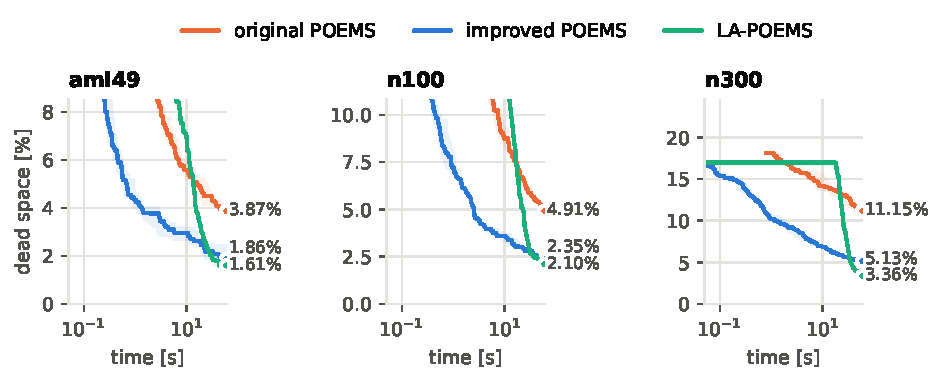
\includegraphics[width=\textwidth]{new/convergence}
\caption{Convergence of the three algorithms on ami49, n100 and n300: median dead space of the best floorplan found so far over the 8 runs (seeds 101--108), with the interquartile range shaded; logarithmic time axis}
\label{fig:convergence}
\end{figure}

\begin{table}
\centering
\small
\begin{tabular}{@{}lrrr@{}}
\toprule
Benchmark & target [\%] & improved POEMS & LA-POEMS \\
\midrule
apte & 0.78 & 0.2 & 0.0 \\
xerox & 3.16 & 0.5 & 0.3 \\
hp & 4.58 & 13.7 & 0.1 \\
ami33 & 3.47 & 4.0 & 9.6 \\
ami49 & 3.87 & 2.2 & 15.4 \\
n100 & 4.91 & 2.6 & 23.6 \\
n200 & 10.02 & 1.4 & 21.7 \\
n300 & 11.15 & 0.7 & 24.5 \\
\bottomrule
\end{tabular}
\caption{Median time [s] in which the improved POEMS and LA-POEMS first reach the median final dead space of the original POEMS (the target, 60\,s runs, seeds 101--108; -- = not reached by half of the runs)}
\label{tab:ttt}
\end{table}


\subsection{Long Runs and Published Results}

Table~\ref{tab:literature} puts the results into the context of the original edition and of published results. The comparison with published results is not controlled (Section~\ref{sec:method}): they were obtained on much slower computers, and their times are given only for orientation. Within 60 seconds, LA-POEMS finds on average less dead space than the longest configuration of the original edition ($I = 20\,000$ iterations), which ran for 12 to 153 minutes on a computer about 1.7 times slower, on every benchmark except apte, where all algorithms find the same floorplan. Its mean dead space is also lower than that of the hard-block packings of CompaSS \cite{compass}, which are computed within seconds, on every benchmark except apte. The B*-Tree with simulated annealing \cite{btree} reports the areas of its floorplans with two decimals. Computed from them, its dead space on apte and hp equals that of the best floorplans of LA-POEMS within the rounding, and on xerox, ami33 and ami49, LA-POEMS finds smaller floorplans on average. Longer runs pay off on the large instances: in five minutes, LA-POEMS reduces the mean dead space on n100, n200 and n300 by another 26--31\,\% compared with the one-minute runs with the same seeds, to 1.66, 2.03 and 2.38\,\% (significantly). On ami33 and ami49, the differences between the one- and the five-minute runs are not significant; on ami33, the mean of the five-minute runs is even higher (1.20 against 1.02\,\%), although their best run reaches 0.84\,\%. The original edition concluded that POEMS outperforms CompaSS on all benchmarks, which its own results did not support for hp (3.88\,\% in its long run against 2.28\,\%). For LA-POEMS, the claim holds on average over one-minute runs on every benchmark except apte, where both find the same floorplan. Fig.~\ref{fig:floorplans} shows the best floorplans found by LA-POEMS.

\begin{table}
\centering
\small
\begin{tabular}{@{}lcccrcrcr@{}}
\toprule
 & \multicolumn{2}{c}{LA-POEMS} & \multicolumn{2}{c}{original edition} & \multicolumn{2}{c}{CompaSS \cite{compass}} & \multicolumn{2}{c}{B*-Tree SA \cite{btree}} \\
Benchmark & 60\,s & 300\,s & [\%] & time [s] & [\%] & time [s] & [\%] & time [s] \\
\midrule
apte & 0.78 (0.78) & -- & 0.78 & 771 & 0.78 & 0.00 & 0.77 & 7 \\
xerox & 2.32 (2.30) & -- & 2.77 & 723 & 3.91 & 0.26 & 2.48 & 25 \\
hp & 1.62 (1.32) & -- & 3.13 & 800 & 2.28 & 0.81 & 1.35 & 55 \\
ami33 & 1.16 (0.63) & 1.20 (0.84) & 2.29 & 1277 & 4.94 & 6.19 & 9.82 & 3417 \\
ami49 & 1.69 (1.36) & 1.51 (1.07) & 2.56 & 1699 & 4.87 & 6.34 & 3.82 & 4752 \\
n100 & 2.15 (1.95) & 1.66 (1.49) & 2.93 & 3145 & 7.32 & 4.17 & -- & -- \\
n200 & 2.75 (2.47) & 2.03 (1.61) & 4.32 & 6067 & 6.48 & 10.43 & -- & -- \\
n300 & 3.39 (2.90) & 2.38 (2.29) & 4.73 & 9200 & 6.80 & 6.87 & -- & -- \\
\bottomrule
\end{tabular}
\caption{LA-POEMS compared with the original edition and with published results: dead space [\%] of LA-POEMS (mean and best of 8 runs of 60\,s, seeds 101--108, and of 5 runs of 300\,s, seeds 101--105), the mean of 10 runs of the longest configuration of the original edition ($I = 20\,000$, on a 2\,GHz computer), CompaSS \cite{benchmcnc,benchgsrc} (2.8\,GHz Pentium~4) and the B*-Tree with simulated annealing \cite{btree} (computed from the areas reported with two decimals, 200\,MHz Sun Ultra-I); times as reported}
\label{tab:literature}
\end{table}


\begin{figure}
\centering
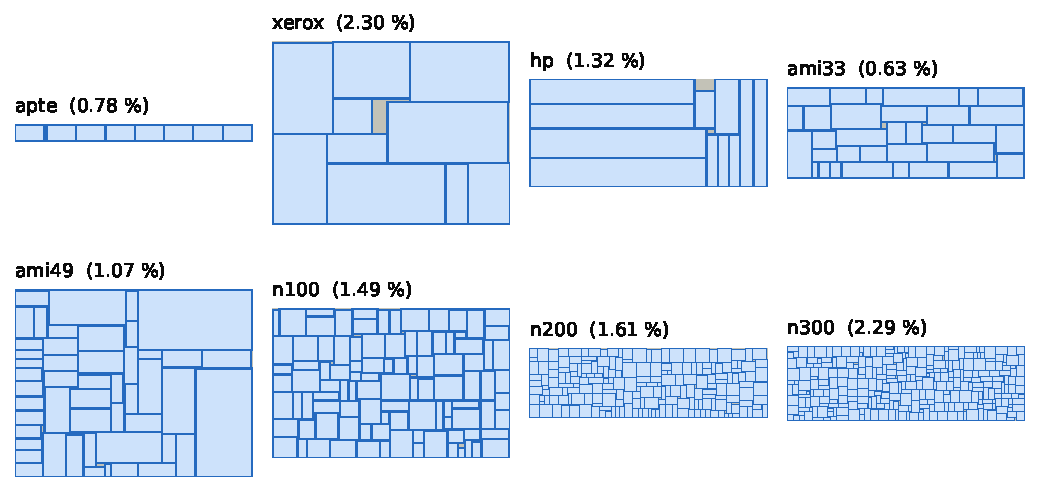
\includegraphics[width=\textwidth]{new/floorplans}
\caption{The best floorplans found by LA-POEMS in the final comparison and in the long runs, with the dead space in gray (the longer side is drawn horizontally). The objective does not constrain the aspect ratio, so some floorplans, such as that of apte, are long strips}
\label{fig:floorplans}
\end{figure}

\paragraph{Answer to RQ4.} With the same time budget of one minute and new seeds, both new algorithms are much better than the original POEMS. The improved POEMS reduces its mean dead space by 44--58\,\% on the tuning instances with 11 or more modules, and LA-POEMS by 57--73\,\% on those with 33 or more modules. LA-POEMS is significantly better than the improved POEMS on five of the seven non-trivial tuning benchmarks and on four of the six held-out instances, and it is not significantly worse on any instance. The advantage has a price: with simulated annealing, the best floorplan improves mainly in the second half of the run, so the time budget must be known in advance. Five-minute runs reduce the dead space on the three largest instances by another 26--31\,\%. Within one minute, LA-POEMS finds on average less dead space than the original edition after up to 2.5 hours and than the published results of CompaSS on every benchmark except apte, where all algorithms find the same floorplan; compared with the B*-Tree with simulated annealing, its best floorplans are equal on apte and hp and smaller on the other three MCNC benchmarks.
